
\documentclass[crop,tikz]{standalone}
\usepackage[utf8]{inputenc}
\usepackage{tikz}
\usepackage{pgfplots}
\pgfplotsset{compat=newest}
\usepgfplotslibrary{groupplots}
\begin{document}
% This file was created by matplotlib2tikz v0.6.15.
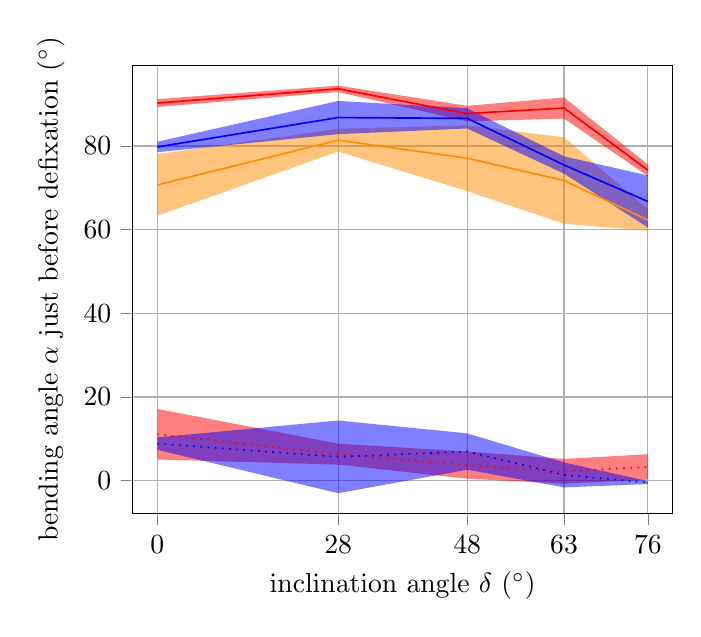
\begin{tikzpicture}

\definecolor{color0}{rgb}{1,0.549019607843137,0}

\begin{axis}[
xlabel={inclination angle $\delta$ ($^\circ$)},
ylabel={bending angle $\alpha$ just before defixation ($^\circ$)},
xmin=-3.8, xmax=79.8,
ymin=-7.87313145155086, ymax=99.2877542677437,
tick align=outside,
tick pos=left,
xmajorgrids,
x grid style={lightgray!92.026143790849673!black},
ymajorgrids,
y grid style={lightgray!92.026143790849673!black},
xtick={0, 28, 48, 63, 76}
]
\path [fill=red, fill opacity=0.5] (axis cs:0,89.3108632973758)
--(axis cs:0,91.1927386978303)
--(axis cs:28,94.4168049168667)
--(axis cs:48,89.5981723047534)
--(axis cs:63,91.5977933707735)
--(axis cs:76,75.5793117892908)
--(axis cs:76,72.8150641609561)
--(axis cs:76,72.8150641609561)
--(axis cs:63,86.5402661873928)
--(axis cs:48,85.8866243592078)
--(axis cs:28,92.9004848613065)
--(axis cs:0,89.3108632973758)
--cycle;

\path [fill=color0, fill opacity=0.5] (axis cs:0,63.3103456358201)
--(axis cs:0,78.0535829182683)
--(axis cs:28,84.0916718987107)
--(axis cs:48,84.9482238860497)
--(axis cs:63,82.0728561774689)
--(axis cs:76,64.8392561713062)
--(axis cs:76,59.7231265717633)
--(axis cs:76,59.7231265717633)
--(axis cs:63,61.4102957608033)
--(axis cs:48,69.2009818046499)
--(axis cs:28,78.6671569708144)
--(axis cs:0,63.3103456358201)
--cycle;

\path [fill=blue, fill opacity=0.5] (axis cs:0,78.5125314409266)
--(axis cs:0,81.0149261206704)
--(axis cs:28,90.759302998606)
--(axis cs:48,89.0124205282408)
--(axis cs:63,77.5167233740239)
--(axis cs:76,72.9428370328851)
--(axis cs:76,60.5168704033792)
--(axis cs:76,60.5168704033792)
--(axis cs:63,73.3853999339688)
--(axis cs:48,84.1828871581441)
--(axis cs:28,82.8179486331038)
--(axis cs:0,78.5125314409266)
--cycle;

\path [fill=red, fill opacity=0.5] (axis cs:0,5.04723465211582)
--(axis cs:0,17.1463232819709)
--(axis cs:28,8.83026784724796)
--(axis cs:48,6.96723325040002)
--(axis cs:63,5.17877796923663)
--(axis cs:76,6.3156037185077)
--(axis cs:76,0.249951975085065)
--(axis cs:76,0.249951975085065)
--(axis cs:63,-0.722952162541954)
--(axis cs:48,0.459741050618337)
--(axis cs:28,3.83299131810499)
--(axis cs:0,5.04723465211582)
--cycle;

\path [fill=blue, fill opacity=0.5] (axis cs:0,7.36982379358714)
--(axis cs:0,10.3349812347311)
--(axis cs:28,14.3750712958308)
--(axis cs:48,11.3018263844633)
--(axis cs:63,4.35166121628628)
--(axis cs:76,-0.104551260956718)
--(axis cs:76,-0.806230637313082)
--(axis cs:76,-0.806230637313082)
--(axis cs:63,-1.60812753177016)
--(axis cs:48,2.61151428803442)
--(axis cs:28,-3.00218210067384)
--(axis cs:0,7.36982379358714)
--cycle;

\addplot [semithick, red, forget plot]
table {%
0 90.2518009976031
28 93.6586448890866
48 87.7423983319806
63 89.0690297790831
76 74.1971879751235
};
\addplot [semithick, color0, forget plot]
table {%
0 70.6819642770442
28 81.3794144347626
48 77.0746028453498
63 71.7415759691361
76 62.2811913715348
};
\addplot [semithick, blue, forget plot]
table {%
0 79.7637287807985
28 86.7886258158549
48 86.5976538431924
63 75.4510616539963
76 66.7298537181322
};
\addplot [semithick, red, dotted, forget plot]
table {%
0 11.0967789670434
28 6.33162958267647
48 3.71348715050918
63 2.22791290334734
76 3.28277784679638
};
\addplot [semithick, blue, dotted, forget plot]
table {%
0 8.85240251415913
28 5.68644459757849
48 6.95667033624884
63 1.37176684225806
76 -0.4553909491349
};
\end{axis}

\end{tikzpicture}
%% End matplotlib2tikz content %% 
\end{document}